\chapter{Transport layer}\label{sec:transport}

This chapter defines the transport layer of Cyphal.
First, the core abstract concepts are introduced.
Afterwards, they are concretized for each supported underlying transport protocol (e.g., CAN bus);
such concretizations are referred to as \emph{concrete transports}.

When referring to a concrete transport, the notation ``Cyphal/X'' is used,
where \emph{X} is the name of the underlying transport protocol.
For example, ``Cyphal/CAN'' refers to CAN bus.

As the specification is extended to add support for new concrete transports,
some of the generic aspects may be pushed to the concrete sections
if they are found to map poorly onto the newly supported protocols.
Such changes are guaranteed to preserve full backward compatibility of the existing concrete transports.

% Please keep \clearpage in front of every section to enforce clear separation!
\clearpage\section{Abstract concepts}

The function of the transport layer is to facilitate exchange of serialized representations of DSDL objects\footnote{%
    DSDL and data serialization are reviewed in chapter~\ref{sec:dsdl}.
} between Cyphal nodes over the \emph{transport network}.

\subsection{Transport model}\label{sec:transport_model}

This section introduces an abstract implementation-agnostic model of the Cyphal transport layer.
The core relations are depicted in figure~\ref{fig:transport_model}.
Some of the concepts introduced at this level may not be manifested in the design of concrete transports;
despite that, they are convenient for an abstract discussion.

% Please do not remove the hard placement specifier [H], it is needed to keep elements ordered.
\begin{figure}[H]
    \centering
    \resizebox{\textwidth}{!}{
        \footnotesize
        \begin{tabu}{|l l l|X[c,2] X[c] X[c]|l|}\hline\rowfont{\bfseries}
            \multicolumn{3}{|c|}{Taxonomy} &
            Message transfers &
            \multicolumn{2}{|c|}{Service transfers} &
            Description \\\hline

            % TRANSFER PAYLOAD
            \multicolumn{3}{|c|}{Transfer payload} &
            \multicolumn{3}{c|}{\bfseries{} Serialized object} &
            The serialized instance of a specific DSDL data type. \\\hline

            % TRANSFER PRIORITY
            \multicolumn{1}{|c|}{\multirow{7}{*}{\rotatebox[origin=c]{90}{Transfer metadata}}} &
            &
            &
            \multicolumn{3}{c|}{\bfseries{} Transfer priority} &
            Defines the urgency (time sensitivity) of the transferred object.\\\cline{4-7}

            % TRANSFER ID
            \multicolumn{1}{|c|}{} &
            &
            &
            \multicolumn{3}{c|}{\bfseries{} Transfer-ID} &
            An integer that uniquely identifies a transfer within its session.\\\cline{2-7}

            % ROUTE SPECIFIER
            \multicolumn{1}{|c|}{} &
            \multicolumn{1}{c|}{\multirow{5}{*}{\rotatebox[origin=c]{90}{\shortstack{Session \\ specifier}}}} &
            \multirow{2}{*}{\shortstack{Route \\ specifier}} &
            \multicolumn{3}{c|}{\bfseries{} Source node-ID} &
            Source node-ID is not specified for anonymous transfers. \\\cline{5-6}

            \multicolumn{1}{|c|}{} &
            \multicolumn{1}{c|}{} &
            &
            \multicolumn{1}{c|}{} &
            \multicolumn{2}{c|}{\bfseries{} Destination node-ID} &
            Destination node-ID is not specified for broadcast transfers.\\\cline{3-7}

            % DATA SPECIFIER
            \multicolumn{1}{|c|}{} &
            \multicolumn{1}{c|}{} &
            \multirow{3}{*}{\shortstack{Data \\ specifier}} &
            \multicolumn{1}{c|}{\multirow{2}{*}{\bfseries{} Subject-ID}} &
            \multicolumn{2}{c|}{\bfseries{} Service-ID} &
            Port-ID specifies how the serialized object should be processed.\\\cline{5-6}

            \multicolumn{1}{|c|}{} &
            \multicolumn{1}{c|}{} &
            &
            \multicolumn{1}{c|}{} &
            {\bfseries{} Request} &
            {\bfseries{} Response} &
            Request/response specifier applies to services only.\\\cline{4-6}

            \multicolumn{1}{|c|}{} &
            \multicolumn{1}{c|}{} &
            &
            \multicolumn{3}{c|}{\bfseries{} Transfer kind} &
            Message (subject) or service transfer.\\\hline
        \end{tabu}
    }
    \caption{Cyphal transport layer model}\label{fig:transport_model}
\end{figure}

\subsubsection{Transfer}

A \emph{transfer} is a singular act of data transmission from one Cyphal node to zero or more other Cyphal nodes
over the transport network.
A transfer carries zero or more bytes of \emph{transfer payload} together with the associated \emph{transfer metadata},
which encodes the semantic and temporal properties of the carried payload.
The elements comprising the metadata are reviewed below.

Transfers are distinguished between \emph{message transfers} and \emph{service transfers} depending on the kind
of the carried DSDL object.
Service transfers are further differentiated between \emph{service request transfers},
which are sent from the invoking node -- \emph{client node} -- to the node that provides the service --
\emph{server node}, and \emph{service response transfers},
which are sent from the server node to the client node upon handling the request.

A transfer is manifested on the transport network as one or more \emph{transport frames}.
A transport frame is an atomic entity carrying the entire transfer payload or a fraction thereof
with the associated transfer metadata --
possibly extended with additional elements specific to the concrete transport --
over the transport network.
The exact definition of a transport frame and the mapping of the abstract transport model onto it
are specific to concrete transports\footnote{
    For example, Cyphal/CAN (introduced later) defines a particular CAN frame format.
    Frames that follow the format are Cyphal transport frames of Cyphal/CAN.
}.

\subsubsection{Transfer payload}\label{sec:transport_transfer_payload}

The transfer payload contains the serialized representation of the carried
DSDL object\footnote{Chapter~\ref{sec:dsdl}.}.

Concrete transports may extend the payload with zero-valued \emph{padding bytes} at the end
to meet the transport-specific data granularity constraints.
Usage of non-zero-valued padding bytes is prohibited for all implementations\footnote{%
    Non-zero padding bytes are disallowed because they would interfere with the implicit zero extension rule
    (section~\ref{sec:dsdl_data_serialization}).
}.

Concrete transports may extend the payload with a \emph{transfer CRC}
-- an additional metadata field used for validating its integrity.
The details of its implementation are dictated by the concrete transport specification.

The deterministic nature of Cyphal in general and DSDL in particular allows implementations to statically determine
the maximum amount of memory that is required to contain the serialized representation
of a DSDL object of a particular type.
Consequently, an implementation that is interested in receiving data objects of a particular type
can statically determine the maximum length of the transfer payload.

Implementations should handle incoming transfers containing a larger amount of payload data than expected.
In the event of such extra payload being received, a compliant implementation should
discard the excessive (unexpected) data at the end of the received payload\footnote{%
    Such occurrence is not indicative of a problem so it should not be reported as such.
}.
The transfer CRC, if applicable, shall be validated regardless of the presence of the extra payload in the transfer.
See figure~\ref{fig:transport_payload_truncation}.

A \emph{transport-layer maximum transmission unit} (MTU) is the maximum amount of data with the associated metadata
that can be transmitted per transport frame for a particular concrete transport.
All nodes connected to a given transport network should share the same transport-layer MTU setting\footnote{%
    Failure to follow this rule may render nodes unable to communicate if a transmitting node emits larger transport
    frames than the receiving node is able to accept.
}.

In order to facilitate the implicit zero extension rule introduced in section~\ref{sec:dsdl_data_serialization},
implementations shall not discard a transfer even if it is determined that it contains less payload
data than a predicted minimum.

A transfer whose payload exceeds the capacity of the transport frame is manifested on the transport network
as a set of multiple transport frames; such transfers are referred to as \emph{multi-frame transfers}.
Implementations shall minimize the number of transport frames constituting a multi-frame transfer by ensuring that
their payload capacity is not underutilized.
Implementations should minimize the delay between transmission of transport frames that belong to the same transfer.
Transport frames of a multi-frame transfer shall be transmitted following the order of the
transfer payload fragments they contain.

A transfer whose payload does not exceed the capacity of the transport frame shall be manifested on the transport
network as a single transport frame\footnote{%
    In other words, multi-frame transfers are prohibited for payloads that can be transferred
    using a single-frame transfer.
}; such transfers are referred to as \emph{single-frame transfers}.

\begin{figure}[H]
    $$
    \raisebox{1em}{\footnotesize{\text{first byte}}}
    \overbrace{%
        \underbrace{%
            \blacksquare\blacksquare\blacksquare\blacksquare\blacksquare\blacksquare%
            \blacksquare\blacksquare\blacksquare\blacksquare\blacksquare\blacksquare%
        }_{\substack{\text{Expected, accepted} \\ \text{payload}}}%
        \underbrace{%
            \boxtimes\boxtimes\boxtimes\boxtimes\boxtimes\boxtimes\boxtimes\boxtimes%
        }_{\substack{\text{Excessive, discarded} \\ \text{payload}}}%
    }^{\substack{%
        \text{Transfer CRC is validated} \\
        \text{for the entire transfer payload} \\
        \text{before the truncation}}
    }
    \raisebox{1em}{\footnotesize{\text{last byte}}}
    $$
    \caption{Transfer payload truncation\label{fig:transport_payload_truncation}}
\end{figure}

\begin{remark}[breakable]
    The requirement to discard the excessive payload data at the end of the transfer is motivated by
    the necessity to allow extensibility of data type definitions, as described in chapter~\ref{sec:dsdl}.
    Additionally, excessive payload data may contain zero padding bytes if required by the concrete transport.

    Let node $A$ publish an object of the following type over the subject $x$:

    \begin{minted}{python}
        float32 parameter
        float32 variance
    \end{minted}

    Let node $B$ subscribe to the subject $x$ expecting an object of the following type:

    \begin{minted}{python}
        float32 parameter
    \end{minted}

    The payload truncation requirement guarantees that the two nodes will be able to interoperate despite
    relying on incompatible data type definitions.
    Under this example, the duty of ensuring the semantic compatibility lies on the system integrator.

    The requirement that all involved nodes use the same transport-layer MTU is crucial here.
    Suppose that the MTU expected by the node $B$ is four bytes and the MTU of the node $A$ is eight bytes.
    Under this setup, messages emitted by $A$ would be contained in single-frame transfers that are too large
    for $B$ to process, resulting in the nodes being unable to communicate.
    An attempt to optimize the memory utilization of $B$ by relying on the fact that the maximum length of a
    serialized representation of the message is four bytes would be a mistake, because this assumption ignores
    the existence of subtyping and introduces leaky abstractions throughout the protocol stack.
\end{remark}

\begin{remark}[breakable]
    The implicit zero extension rule makes deserialization routines sensitive to the trailing unused data.
    For example, suppose that a publisher emits an object of type:

    \begin{minted}{python}
        uint16 foo
    \end{minted}

    Suppose that the concrete transport at hand requires padding to 4 bytes, which is done with $55_{16}$
    (intentionally non-compliant for the sake of this example).
    Suppose that the published value is $1234_{16}$,
    so the resulting serialized representation is $\left[34_{16}, 12_{16}, 55_{16}, 55_{16}\right]$.
    Suppose that the receiving side relies on the implicit zero extension rule with the following definition:

    \begin{minted}{python}
        uint16 foo
        uint16 bar
    \end{minted}

    The expectation is that \verb|foo| will be deserialized as $1234_{16}$,
    and \verb|bar| will be zero-extended as $0000_{16}$.
    If arbitrary padding values were allowed, the value of \verb|bar| would become undefined;
    in this particular example it would be $5555_{16}$.

    Therefore, the implicit zero-extension rule requires that padding is done with zero bytes only.
\end{remark}

\subsubsection{Transfer priority}\label{sec:transport_transfer_priority}

Transfers are prioritized by means of the \emph{transfer priority} parameter,
which allows at least 8 (eight) distinct priority levels.
Concrete transports may support more than eight priority levels.

Transmission of transport frames shall be ordered so that frames of higher priority are transmitted first.
It follows that higher-priority transfers may preempt transmission of lower-priority transfers.

Transmission of transport frames that share the same priority level should follow the order of their appearance in
the transmission queue.

Priority of message transfers and service request transfers can be chosen freely
according to the requirements of the application.
Priority of a service response transfer should match the priority of the corresponding service request transfer.

\begin{remark}[breakable]
    Transfer prioritization is paramount for distributed real-time applications.

    The priority level mnemonics and their usage recommendations are specified in the following list.
    The mapping between the mnemonics and actual numeric identifiers is transport-dependent.

    % https://forum.opencyphal.org/t/transfer-priority-level-mnemonics/218/6?u=pavel.kirienko
    \begin{description}
        \item[Exceptional] -- The bus designer can ignore these messages when calculating bus load since they
        should only be sent when a total system failure has occurred.
        For example, a self-destruct message on a rocket would use this priority.
        Another analogy is an NMI on a microcontroller.

        \item[Immediate] -- Immediate is a ``high priority message'' but with additional latency constraints.
        Since exceptional messages are not considered when designing a bus, the latency of immediate messages
        can be determined by considering only immediate messages.

        \item[Fast] -- Fast and immediate are both ``high priority messages'' but with additional latency constraints.
        Since exceptional messages are not considered when designing a bus,
        the latency of fast messages can be determined by considering only immediate and fast messages.

        \item[High] -- High priority messages are more important than nominal messages but have looser
        latency requirements than fast messages. This priority is used so that,
        in the presence of rogue nominal messages, important commands can be received.
        For example, one might envision a failure mode where a temperature sensor starts to
        load a vehicle bus with nominal messages.
        The vehicle remains operational (for a time) because the controller is exchanging fast and
        immediate messages with sensors and actuators.
        A system safety monitor is able to detect the distressed bus and command the vehicle to a
        safe state by sending high priority messages to the controller.

        \item[Nominal] -- This is what all messages should use by default.
        Specifically the heartbeat messages should use this priority.

        \item[Low] -- Low priority messages are expected to be sent on a bus under all conditions but cannot
        prevent the delivery of nominal messages.
        They are allowed to be delayed but latency should be constrained by the bus designer.

        \item[Slow] -- Slow messages are low priority messages that have no time sensitivity at all.
        The bus designer need only ensure that, for all possible system states,
        these messages will eventually be sent.

        \item[Optional] -- These messages might never be sent (theoretically) for some possible system states.
        The system shall tolerate never exchanging optional messages in every possible state.
        The bus designer can ignore these messages when calculating bus load.
        This should be the priority used for diagnostic or debug messages that are not required on an
        operational system.
    \end{description}
\end{remark}

\subsubsection{Route specifier}\label{sec:transport_route_specifier}

The \emph{route specifier} defines the node-ID of the origin and the node-ID of the destination of a transfer.

A \emph{broadcast transfer} is a transfer that does not have a specific destination;
the decision of whether to process a broadcast transfer is delegated to receiving nodes\footnote{%
    This does not imply that applications are required to be involved with every broadcast transfer.
    The opt-in logic is facilitated by the low-level routing and/or filtering features implemented
    by the network stack and/or the underlying hardware.
}.
A \emph{unicast transfer} is a transfer that is addressed to a specific single node\footnote{%
    Whose existence and availability is optional.
} whose node-ID is not the same as that of the origin;
which node should process a unicast transfer is decided by the sending node.

A node that does not have a node-ID is referred to as \emph{anonymous node}.
Such nodes are unable to emit transfers other than \emph{anonymous transfers}.
An anonymous transfer is a transfer that does not have a specific source.
Anonymous transfers have the following limitations\footnote{%
    Anonymous transfers are intended primarily for the facilitation of the optional plug-and-play feature
    (section~\ref{sec:application_functions})
    which enables fully automatic configuration of Cyphal nodes upon their connection to the network.
    Some transports may provide native support for auto-configuration, rendering anonymous transfers unnecessary.
}:
\begin{itemize}
    \item An anonymous transfer can be only a message transfer.
    \item An anonymous transfer can be only a single-frame transfer.
    \item Concrete transports may introduce arbitrary additional restrictions
          on anonymous transfers or omit their support completely.
\end{itemize}

A message transfer can be only a broadcast transfer; unicast message transfers are not defined\footnote{%
    Unicast message transfers may be defined in a future revision of this Specification.
}.
A service transfer can be only a unicast transfer; broadcast service transfers are prohibited.

\begin{CyphalCompactTable}{|l l l|}
    Transfer kind       & Unicast       & Broadcast     \\
    Message transfer    & Not defined   & Valid         \\
    Service transfer    & Valid         & Prohibited    \\
\end{CyphalCompactTable}

\subsubsection{Data specifier}\label{sec:transport_data_specifier}

The \emph{data specifier} encodes the semantic properties of the DSDL object carried by a transfer and its kind.

The data specifier of a message transfer is the subject-ID of the contained DSDL message object.

The data specifier of a service transfer is a combination of the service-ID of the contained DSDL service object
and an additional binary parameter that segregates service requests from service responses.

\subsubsection{Session specifier}\label{sec:transport_session_specifier}

The \emph{session specifier} is a combination of the data specifier and the route specifier.
Its function is to uniquely identify a category of transfers by the semantics of exchanged data and
the agents participating in its exchange while abstracting over individual transfers and their concrete data\footnote{%
    Due to the fact that anonymous transfers lack information about their origin,
    all anonymous transfers that share the same data specifier and destination
    are grouped under the same session specifier.
}.

The term \emph{session} used here denotes the node's local representation of a logical communication
channel that it is a member of.
Following the stateless and low-context nature of Cyphal, this concept excludes any notion of explicit state sharing
between nodes.

\begin{remark}[breakable]
    One of the key design principles is that Cyphal is a stateless low-context protocol where collaborating agents
    do not make strong assumptions about the state of each other.
    Statelessness and context invariance are important because they facilitate behavioral simplicity and robustness;
    these properties are desirable for deterministic real-time distributed applications which Cyphal is designed for.

    Design and verification of a system that relies on multiple agents sharing the same model of a distributed process
    necessitates careful analysis of special cases such as unintended state divergence, latency and transient states,
    sudden loss of state (e.g., due to disconnection or a software reset), etc.
    Lack of adequate consideration may render the resulting solution fragile and prone to unspecified behaviors.

    Some of the practical consequences of the low-context design include the ability of a node to immediately
    commence operation on the network without any prior initialization steps.
    Likewise, addition and removal of a subscriber to a given subject is transparent to the publisher.

    The above considerations only hold for the communication protocol itself.
    Applications whose functionality is built on top of the protocol may engage in state sharing if such is
    found to be beneficial\footnote{%
        Related discussion in
        \url{https://forum.opencyphal.org/t/idempotent-interfaces-and-deterministic-data-loss-mitigation/643}.
    }.
\end{remark}

\begin{remark}[breakable]
    Some implementations of the Cyphal communication stack may contain states indexed by the session specifier.
    For example, in order to emit a transfer, the stack may need to query the appropriate transfer-ID counter
    (section~\ref{sec:transport_transfer_id}) by the session specifier of the transfer.
    Likewise, in order to process a received frame,
    the stack may need to locate the appropriate states keyed by the session specifier.

    Given the intended application domains of Cyphal,
    the temporal characteristics of such look-up activities should be well-characterized and predictable.
    Due to the fact that all underlying primitive parameters that form the session specifier
    (such as node-ID, port-ID, etc.) have statically defined bounds,
    it is trivial to construct a look-up procedure satisfying any computational complexity envelope,
    from constant-complexity $O(1)$ at the expense of heightened memory utilization,
    up to low-memory-footprint $O(n)$ if temporal predictability is less relevant.

    For example, given a subject-ID, the maximum number of distinct sessions that can be observed
    by the local node will never exceed the number of nodes in the network minus one\footnote{%
        A node cannot receive transfers from itself, hence minus one.
    }.
    If the number of nodes in the network cannot be reliably known in advance (which is the case in most applications),
    it can be considered to equal the maximum number of nodes permitted by the concrete transport\footnote{%
        E.g., 128 nodes for the CAN bus transport.
    }.
    The total number of distinct sessions that can be observed by a node is a product of the number
    of distinct data specifiers utilized by the node and the number of other nodes in the network.

    It is recognized that highly rigid safety-critical applications may benefit from avoiding any
    dynamic look-up by sacrificing generality, by employing automatic code generation, or through other methods,
    in the interest of greater determinism and robustness.
    In such cases, the above considerations may be irrelevant.
\end{remark}

\subsubsection{Transfer-ID}\label{sec:transport_transfer_id}

The \emph{transfer-ID} is an unsigned integer value that is provided for every transfer.
Barring the case of transfer-ID overflow reviewed below,
each transfer under a given session specifier has a unique transfer-ID value.
This parameter is crucial for many aspects of Cyphal communication\footnote{%
    One might be tempted to use the transfer-ID value for temporal synchronization of
    parallel message streams originating from the same node,
    where messages bearing the same transfer-ID value are supposed to correspond to the same moment in time.
    Such use is strongly discouraged because it is incompatible with transports that rely on overflowing
    transfer-ID values and because it introduces a leaky abstraction into the system.
    If temporal synchronization is necessary, explicit time stamping should be used instead.
}; specifically:

\begin{description}
    \item[Message sequence monitoring] -- transfer-ID allows receiving nodes to detect discontinuities
    in incoming message streams from remote nodes.

    \item[Service response matching] -- when a server responds to a request, it uses the same transfer-ID for the
    response transfer as in the request transfer,
    allowing the client to emit concurrent requests to the same server while being able to
    match each response with the corresponding local request state.

    \item[Transfer deduplication] -- the transfer-ID allows receiving nodes to detect and eliminate duplicated
    transfers.
    Transfer duplication may occur either spuriously as an artifact of a concrete transport\footnote{%
        For example, in CAN bus, a frame that appears valid to the receiver may under certain (rare) conditions
        appear invalid to the transmitter, triggering the latter to retransmit the frame,
        in which case it will be duplicated on the side of the receiver.
        Sequence counting mechanisms such as transfer-ID allow implementations to circumvent this problem.
    } or deliberately as a method of deterministic data loss mitigation for unreliable links
    (section~\ref{sec:transport_deterministic_data_loss_mitigation}).

    \item[Multi-frame transfer reassembly] -- a transfer that is split over multiple transport frames is reassembled
    back upon reception with the help of transfer-ID: all transport frames that comprise a transfer
    share the same transfer-ID value.

    \item[Automatic management of redundant interfaces] -- in redundant transport networks,
    transfer-ID enables automatic switchover to a back-up interface shall the primary interface fail.
    The switchover logic can be completely transparent to the application, joining several independent
    redundant transport networks into a highly reliable single virtual communication channel.
\end{description}

For service response transfers the transfer-ID value shall be directly copied from the corresponding
service request transfer\footnote{This behavior facilitates request-response matching on the client node.}.

A node that is interested in emitting message transfers or service request transfers
under a particular session specifier, whether periodically or on an ad-hoc basis,
shall allocate a transfer-ID counter state associated with said session specifier exclusively.
The transfer-ID value of every emitted transfer is determined by sampling the corresponding counter
keyed by the session specifier of the transfer; afterwards, the counter is incremented by one.

When the transfer-ID counter reaches the maximum value defined for the concrete transport,
the next increment resets its value to zero.
Transports where the number of distinct transfer-ID values is not less than $2^{48}$ are said to have
\emph{monotonic transfer-ID}.
Those with narrower transfer-ID counters are said to have \emph{cyclic transfer-ID};
the number of unique transfer-ID values is referred to as \emph{transfer-ID modulo}.

The initial value of a cyclic transfer-ID counter shall be zero.
The initial value of a monotonic transfer-ID counter should be zero.
Once a new transfer-ID counter is created,
it should be kept at least as long as the node remains connected to the network.\footnote{%
    The number of unique session specifiers is bounded and can be determined statically per application,
    so this requirement does not introduce non-deterministic features into the application even if it leverages
    aperiodic/ad-hoc transfers.
}.

\emph{Transfer-ID difference} for a pair of transfer-ID values $a$ and $b$ is defined
for monotonic transfer-ID as their arithmetic difference $a-b$.
For a cyclic transfer-ID, the difference is defined as the number of increment operations that need to be applied
to $b$ so that $a = b^\prime{}$.

\begin{remark}
    A C++ implementation of the cyclic transfer-ID difference operator is provided here.
    \begin{minted}{cpp}
        #include <cstdint>
        /**
         * Cyphal cyclic transfer-ID difference computation algorithm implemented in C++.
         * License: CC0, no copyright reserved.
         * @param a         Left-hand operand (minuend).
         * @param b         Right-hand operand (subtrahend).
         * @param modulo    The number of distinct transfer-ID values, or the maximum value plus one.
         * @returns         The number of increment operations separating b from a.
         */
        [[nodiscard]]
        constexpr std::uint8_t computeCyclicTransferIDDifference(const std::uint8_t a,
                                                                 const std::uint8_t b,
                                                                 const std::uint8_t modulo)
        {
            std::int16_t d = static_cast<std::int16_t>(a) - static_cast<std::int16_t>(b);
            if (d < 0)
            {
                d += static_cast<std::int16_t>(modulo);
            }
            return static_cast<std::uint8_t>(d);
        }
    \end{minted}
\end{remark}

\subsection{Redundant transports}

Cyphal supports transport redundancy for the benefit of a certain class of safety-critical applications.
A redundant transport interconnects nodes belonging to the same network (all or their subset)
via more than one transport network.
A set of such transport networks that together form a redundant transport is referred to as a
\emph{redundant transport group}.

Each member of a redundant transport group shall be capable of independent operation
such that the level of service of the resulting redundant transport remains constant
as long as at least one member of the redundant group remains functional\footnote{%
    Redundant transports are designed for increased fault tolerance, not for load sharing.
}.

\begin{remark}
    Networks containing nodes with different reliability requirements may benefit from
    nonuniform redundant transport configurations, where non-critical nodes are interconnected
    using a lower number of transports than critical nodes.

    Designers should recognize that nonuniform redundancy may complicate the analysis of the network.
\end{remark}

% The following fragment deals with heterogeneous transports.
% Its inclusion in the body of the document does not make sense until the UDP/IP and Serial transports
% (and/or other transports) are formally specified. When they are, this fragment will be uncommented.
\begin{comment}
\subsubsection{Heterogeneous redundant transports}

A \emph{heterogeneous redundant transport} is a redundant transport configuration where nodes are
interconnected using different concrete transports.
Heterogeneous transports may facilitate higher fault tolerance provided that the failure modes of involved transports
are sufficiently dissimilar\footnote{%
    Consider a heterogeneous configuration combining wired and wireless transports.
    See also ``Wireless Avionics Intra-Communications'' (WAIC).
}.
A heterogeneous redundant transport shall meet \emph{either} of the following requirements:
\begin{itemize}
    \item All of the involved transports shall use monotonic transfer-ID\footnote{%
              Section~\ref{sec:transport_transfer_id}.
          }.
          In this case, the resulting redundant transport is said to be a monotonic transfer-ID transport as well.

    \item All of the involved transports shall use cyclic transfer-ID with identical value ranges.
          In this case, the resulting redundant transport is said to be a cyclic transfer-ID transport as well.
\end{itemize}

\begin{remark}[breakable]
    Transports with monotonic transfer-ID have a higher metadata overhead per frame due to the requirement
    to accommodate a sufficiently wide integer field for the transfer-ID value.
    Their advantage is that transfer-ID values of all transports in a redundant group
    are guaranteed to remain in-phase as long as the node is running.
    The importance of this guarantee can be demonstrated with the following counterexample
    of two transports leveraging different transfer-ID ranges for the same session,
    where the unambiguous mapping between their transfer-ID values is lost after the first overflow
    (figure~\ref{fig:transport_cyclic_transfer_id_redundant}).

    % Plot[{
    %   Mod[x, 40],
    %   Mod[x, 32]
    %  },
    %  {x, 0, 150},
    %  PlotLegends -> {"[0,40]", "[0,32]"},
    %  GridLines -> {{}, {32, 40}},
    %  AxesLabel -> {"Count", "Transfer-ID"},
    %  Epilog -> {
    %    Text["Epoch 0", {20, 35}],
    %    Text["Epoch 1", {60, 35}],
    %    Text["Epoch 2", {100, 35}],
    %    Text["Epoch 3", {140, 35}]
    %   }
    %  ]
    \begin{figure}[H]
        \centering
        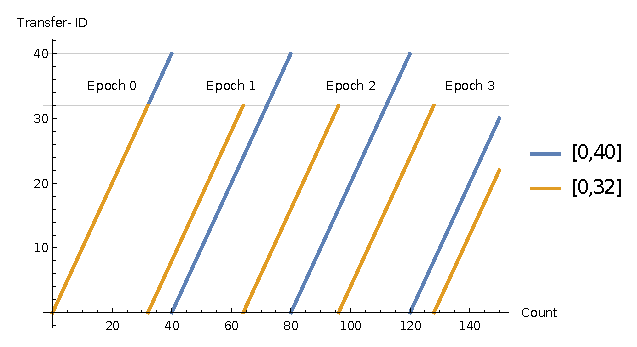
\includegraphics[width=0.6\textwidth]{transport/cyclic_transfer_id_redundant_transport}
        \caption{Issues with cyclic transfer-ID in heterogeneous redundant transports}
        \label{fig:transport_cyclic_transfer_id_redundant}
    \end{figure}
\end{remark}
\end{comment}

\subsection{Transfer transmission}

\subsubsection{Transmission timeout}

The transport frames of a time-sensitive transfer whose payload has lost relevance due to
its transmission being delayed should be removed from the transmission queue\footnote{%
    Trailing transport frames of partially transmitted multi-frame transfers should be removed as well.
    The objective of this recommendation is to ensure that obsolete data is not transmitted
    as it may have adverse effects on the system.
}.
The time interval between the point where the transfer is constructed and the point where it is considered
to have lost relevance is referred to as \emph{transmission timeout}.

% "Output port" sounds better but this term is not defined.
The transmission timeout should be documented for each outgoing transfer port.

\subsubsection{Pending service requests}

In the case of cyclic transfer-ID transports (section~\ref{sec:transport_transfer_id}),
implementations should ensure that upon a transfer-ID overflow a service client session
does not reuse the same transfer-ID value for more than one pending request simultaneously.

\subsubsection{Deterministic data loss mitigation}\label{sec:transport_deterministic_data_loss_mitigation}

Performance of transport networks where the probability of a successful transfer delivery
does not meet design requirements can be adjusted by repeating relevant outgoing transfers
under the same transfer-ID value\footnote{%
    Removal of intentionally duplicated transfers on the receiving side is natively guaranteed
    by this transport layer specification;
    no special activities are needed there to accommodate this feature.
}.
This tactic is referred to as \emph{deterministic data loss mitigation}\footnote{%
    Discussed in
    \url{https://forum.opencyphal.org/t/idempotent-interfaces-and-deterministic-data-loss-mitigation/643}.
}.

\subsubsection{Transmission over redundant transports}

Nodes equipped with redundant transports shall submit every outgoing transfer to the transmission queues of all
available redundant transports simultaneously\footnote{%
    The objective of this requirement is to guarantee that a redundant transport remains fully functional
    as long as at least one transport in the redundant group is functional.
}.
It is recognized that perfectly simultaneous transmission may not be possible due to different
utilization rates of the redundant transports, different phasing of their traffic, and/or application constraints,
in which case implementations should strive to minimize the temporal skew as long as that
does not increase the latency.

An exception to the above rule applies if the payload of the transfer is a function of
the identity of the transport instance that carries the transfer\footnote{%
    An example of such a special case is the time synchronization algorithm documented
    in section~\ref{sec:application_functions}.
}.

\subsection{Transfer reception}\label{sec:transport_transfer_reception}

\subsubsection{Definitions}

\emph{Transfer reassembly} is the real-time process of reconstruction of the transfer payload and its metadata from
a sequence of relevant transport frames.

\emph{Transfer-ID timeout} is a time interval whose semantics are explained below.
Implementations may define this value statically according to the application requirements.
Implementations may automatically adjust this value per session at runtime as a function of the
observed transfer reception interval.
Implementations should document the value of transfer-ID timeout or the rules of its computation.

\emph{Transport frame reception timestamp} specifies the moment of time when the frame is received by a node.
\emph{Transfer reception timestamp} is the reception timestamp of the earliest received frame of the transfer.

An \emph{ordered transfer sequence} is a sequence of transfers whose temporal order is
covariant with their transfer-ID values.

\subsubsection{Behaviors}

For a given session specifier, every unique transfer
(differentiated from other transfers in the same session by its transfer-ID)
shall be received at most once\footnote{%
    In other words, intentional and unintentional duplicates shall be removed.
    Intentional duplications are introduced by the deterministic data loss mitigation measure or redundant transports.
    Unintentional duplications may be introduced by various artifacts of the transport network.
}.

For a given session specifier, a successfully reassembled transfer that is
temporally separated from any other successfully reassembled transfer under the same session specifier
by more than the transfer-ID timeout is considered unique regardless of its transfer-ID value.

If the optimal transfer-ID timeout value for a given session cannot be known in advance,
it can be computed at runtime on a per-session basis\footnote{%
    E.g., as a multiple of the average transfer reception interval.
}.
The parameters of such computation are to be chosen according to the requirements of the application,
but they should always be documented.

The transfer-ID timeout used with service response transfers should be zero\footnote{%
    With a non-zero transfer-ID timeout, responses may be lost if the server responds to multiple requests
    from the same client not in the order of their arrival.
    There is no risk of response duplication because the client will retire the pending request entry
    once its first response is received, ignoring subsequent duplicates.
}.

\begin{remark}
    Low transfer-ID timeout values increase the risk of undetected transfer duplication when such transfers
    are significantly delayed due to network congestion,
    which is possible with very low-priority transfers when the network load is high.

    High transfer-ID timeout values increase the risk of an undetected transfer loss
    when a remote node suffers a loss of state (e.g., due to a software reset).

    The ability to auto-detect the optimal transfer-ID timeout value per session at runtime ensures that the
    application can find the optimal balance even if the temporal properties of the network are not known in advance.
    As a practical example, an implementation could compute the exponential moving average of the
    transfer reception interval $x$ for a given session and define the transfer-ID timeout as $2x$.

    It is important to note that the automatic adjustment of the transfer-ID timeout should only be done
    on a per-session basis rather than for the entire port, because there may be multiple remote nodes
    emitting transfers on the same port at different rates.
    For example, if one node emits transfers at a rate $r$ transfers per second, and another node emits transfers
    on the same port at a much higher rate $100r$, the resulting auto-detected transfer-ID timeout might be
    too low, creating the risk of accepting duplicates.
\end{remark}

Implementations are recommended, but not required, to support reassembly of
multi-frame transfers where the temporal ordering of the transport frames is distorted.

\begin{remark}
    For a certain category of transport implementations, reassembly of multi-frame transfers from an
    unordered transport frame sequence increases the probability of successful delivery if
    the probability of a transport frame loss is non-zero and transport frames are intentionally duplicated.

    Such intentional duplication occurs in redundant transports and if deterministic data loss mitigation is used.
    The reason is that the loss of a single transport frame is observed by the receiving node as its relocation
    from its original position in the sequence to the position of its duplicate.
\end{remark}

Reassembled transfers shall form an ordered transfer sequence.

For a cyclic transfer-ID redundant transport whose redundant group contains $n$ transports,
if up to $n-1$ transports in the redundant group lose the ability to exchange transport frames between nodes,
the transfer reassembly process shall be able to restore nominal functionality
in an amount of time that does not exceed the transfer-ID timeout.

\begin{remark}
    Cyclic transfer-ID transport implementations are recommended to insert a delay before performing
    an automatic fail-over.
    As indicated in the normative description, the delay may be arbitrary as long as it does not exceed the
    transfer-ID timeout value.

    The fail-over delay allows implementations to uphold the transfer uniqueness requirement when the phasing of
    traffic on different transports within the redundant group differs by more than the transfer-ID overflow period.
\end{remark}

For a monotonic transfer-ID redundant transport whose redundant group contains $n$ transports,
if up to $n-1$ transports in the redundant group lose the ability to exchange transport frames between nodes,
the performance of the transfer reassembly process shall not be affected.

\begin{remark}
    Monotonic transfer-ID transport implementations are recommended to always accept the first transfer
    to arrive regardless of which transport within the redundant group it was delivered over.

    This behavior ensures that the total latency of a redundant transport equals the latency of the best-performing
    transport within the redundant group (i.e., the total latency equals the latency of the fastest transport).
    Since a monotonic transfer-ID does not overflow, there is no risk of failing to uphold the uniqueness guarantee
    unlike with the case of cyclic transfer-ID.
\end{remark}

If anonymous transfers are supported by the concrete transport,
reassembly of anonymous transfers shall be implemented by unconditional acceptance of their transport frames.
Requirements pertaining to ordering and uniqueness do not apply.

\begin{remark}
    Regardless of the concrete transport in use and its capabilities,
    Cyphal provides the following guarantees (excluding anonymous transfers):

    \begin{itemize}
        \item Removal of duplicates. If a transfer is delivered, it is guaranteed that it is delivered once,
              even if intentionally duplicated by the origin.
        \item Correct ordering. Received transfers are ordered according to their transfer-ID values.
        \item Deterministic automatic fail-over in the event of a failure of a transport (or several)
              in a redundant group.
    \end{itemize}

    For anonymous transfers, ordering and uniqueness are impossible to enforce
    because anonymous transfers that originate from different nodes may share the same session specifier.

    Reassembly of transfers from redundant interfaces may be implemented either on the per-transport-frame level
    or on the per-transfer level.
    The former amounts to receiving individual transport frames from redundant interfaces
    which are then used for reassembly; it can be seen that this method requires that all transports in the
    redundant group use identical application-level MTU (i.e., same number of transfer payload bytes per frame).
    The latter can be implemented by treating each transport in the redundant group separately,
    so that each runs an independent transfer reassembly process, whose outputs are then deduplicated
    on the per-transfer level; this method may be more computationally complex but it provides greater flexibility.
    A detailed discussion is omitted because it is outside of the scope of this specification.
\end{remark}

\clearpage\section{Cyphal/CAN}\label{sec:transport_can}

\hyphenation{Cyphal/CAN}  % Disable hyphenation.

This section specifies a concrete transport based on ISO 11898 CAN bus.
Throughout this section, ``CAN'' implies both Classic CAN 2.0 and CAN FD, unless specifically noted otherwise.
CAN FD should be considered the primary transport protocol.

\begin{CyphalSimpleTable}{Cyphal/CAN transport capabilities}{|l X l|}
    \label{table:transport_can_capabilities}
    Parameter & Value & References \\

    Maximum node-ID value &
    127 (7 bits wide). &
    \ref{sec:basic} \\

    Transfer-ID mode &
    Cyclic, modulo 32. &
    \ref{sec:transport_transfer_id} \\

    Number of transfer priority levels &
    8 (no additional levels). &
    \ref{sec:transport_transfer_priority} \\

    Largest single-frame transfer payload &
    Classic CAN -- 7~bytes, CAN FD -- up to 63~bytes. &
    \ref{sec:transport_transfer_payload} \\

    Anonymous transfers &
    Supported with non-deterministic collision resolution policy. &
    \ref{sec:transport_route_specifier} \\
\end{CyphalSimpleTable}

\subsection{CAN ID field}

Cyphal/CAN transport frames are CAN 2.0B frames.
The 29-bit CAN ID encodes the session specifier\footnote{Section~\ref{sec:transport_session_specifier}.}
of the transfer it belongs to along with its priority.
The CAN data field of every frame contains the transfer payload
(or, in the case of multi-frame transfers, a fraction thereof), the transfer-ID, and other metadata.

Cyphal/CAN can share the same bus with other high-level CAN bus protocols provided that they
do not make use of CAN 2.0B frames\footnote{For example, CANOpen or CANaerospace.}.
However, future revisions of Cyphal/CAN may utilize CAN 2.0A as well,
so backward compatibility with other high-level CAN bus protocols is not guaranteed.

Cyphal/CAN utilizes two different CAN ID bit layouts for message transfers and service transfers.
The bit layouts are summarized on figure~\ref{fig:transport_can_id_structure}.
Tables~\ref{table:transport_can_id_fields_message_transfer} and~\ref{table:transport_can_id_fields_service_transfer}
summarize the purpose of each field and their permitted values
for message transfers and service transfers, respectively.

% Please do not remove the hard placement specifier [H], it is needed to keep elements ordered.
\begin{figure}[H]
    \centering
    \resizebox{\textwidth}{!}{
        \footnotesize
        \begin{tabular}{|l|c|c|c|c|c|c|c|c|c|c|c|c|c|c|c|c|c|c|c|c|c|c|c|c|c|c|c|c|c|} \hline
            %
            % Message transfer
            %
            \multirow{2}{*}{\textbf{Message}} &
            \multicolumn{4}{c|}{Service, not message} &
            \multicolumn{4}{c|}{Anonymous} &
            \multicolumn{13}{c|}{\multirow{2}{*}{Subject-ID}} &
            \multicolumn{1}{c|}{\multirow{2}{*}{R}} &
            \multicolumn{7}{c|}{\multirow{2}{*}{Source node-ID}}
            \\\cline{2-4} \cline{7-9}

            &
            \multicolumn{3}{c|}{Priority}
            &
            &
            &
            R &
            R &
            R &
            \multicolumn{13}{c|}{} &
            &
            \multicolumn{7}{c|}{}
            \\

            \textbf{Values} &
            \multicolumn{3}{c|}{$[0, 7]$} &
            $0$ &
            $\mathbb{B}$ &
            $0$ &
            $1$ &
            $1$ &
            \multicolumn{13}{c|}{$[0, 8191]$} &
            $0$ &
            \multicolumn{7}{c|}{$[0, 127]$}
            \\\hline

            \textbf{CAN ID bit} &
            28 & 27 & 26 & 25 & 24 & 23 & 22 & 21 & 20 & 19 & 18 & 17 & 16 & 15 &
            14 & 13 & 12 & 11 & 10 &  9 &  8 &  7 &  6 &  5 &  4 &  3 &  2 &  1 &  0
            \\\hline

            \textbf{CAN ID byte} &
            \multicolumn{5}{c|}{3} & \multicolumn{8}{c|}{2} & \multicolumn{8}{c|}{1} & \multicolumn{8}{c|}{0}
            \\\hline

            \multicolumn{30}{c}{} \\ \hline % Table separator

            %
            % Service transfer
            %
            \multirow{2}{*}{\textbf{Service}} &
            \multicolumn{4}{c|}{Service, not message} &
            \multicolumn{5}{c|}{Request, not response} &
            \multicolumn{6}{c|}{} &
            \multicolumn{7}{c|}{\multirow{2}{*}{Destination node-ID}} &
            \multicolumn{7}{c|}{\multirow{2}{*}{Source node-ID}}
            \\\cline{2-4} \cline{7-10}

            &
            \multicolumn{3}{c|}{Priority} &
            &
            &
            R &
            \multicolumn{9}{c|}{Service-ID} &
            \multicolumn{7}{c|}{} &
            \multicolumn{7}{c|}{}
            \\

            \textbf{Values} &
            \multicolumn{3}{c|}{$[0, 7]$} &
            $1$ &
            $\mathbb{B}$ &
            $0$ &
            \multicolumn{9}{c|}{$[0, 511]$} &
            \multicolumn{7}{c|}{$[0, 127]$} &
            \multicolumn{7}{c|}{$[0, 127]$}
            \\\hline

            \textbf{CAN ID bit} &
            28 & 27 & 26 & 25 & 24 & 23 & 22 & 21 & 20 & 19 & 18 & 17 & 16 & 15 &
            14 & 13 & 12 & 11 & 10 &  9 &  8 &  7 &  6 &  5 &  4 &  3 &  2 &  1 &  0
            \\\hline

            \textbf{CAN ID byte} &
            \multicolumn{5}{c|}{3} & \multicolumn{8}{c|}{2} & \multicolumn{8}{c|}{1} & \multicolumn{8}{c|}{0}
            \\\hline
        \end{tabular}
    }
    \caption{CAN ID bit layout}\label{fig:transport_can_id_structure}
\end{figure}

\begin{CyphalSimpleTable}[wide]{CAN ID bit fields for message transfers}{|l l l X|}
    \label{table:transport_can_id_fields_message_transfer}
    Field               & Width & Valid values  & Description \\

    Transfer priority   & 3     & $[0, 7]$ (any)    & Section~\ref{sec:transport_transfer_priority}. \\

    Service, not message & 1    & $0$               & Always zero for message transfers. \\

    Anonymous           & 1     & $\{0, 1\}$ (any)  & Zero for regular message transfers,
                                                      one for anonymous transfers. \\

    Reserved bit 23     & 1     & $0$               & Discard frame if this field has a different value. \\

    % The asymmetric requirement to transmit only 1 and accept any value is due to the need to ensure compatibility
    % with the implementations following the v1-alpha spec, where the width of the subject-ID field was 15 bit
    % (two bits wider). We keep the most significant bits set to ensure the compatibility of the regulated subject-IDs
    % between v1-alpha and v1-beta. Ensuring the compatibility of unregulated subject-IDs is far less important because
    % generally, they are easily changeable.
    %
    % Such backward-compatible change renders these two bits unusable for the possible future expansion of the
    % subject-ID field, but this is fine, because shall the expansion become imminent, we can always flip R7 from 0
    % to 1, and thus pave the way for a completely new bit layout format with a wider subject-ID. Meanwhile, R21 and
    % R22 can be leveraged for some additional optional features.
    Reserved bit 22     & 1     & $1$, any          & Transmit $1$; ignore (do not check) when receiving. \\
    Reserved bit 21     & 1     & $1$, any          & Transmit $1$; ignore (do not check) when receiving. \\

    Subject-ID          & 13    & $[0, 8191]$ (any) & Subject-ID of the current message transfer. \\

    Reserved bit 7      & 1     & $0$               & Discard frame if this field has a different value. \\

    Source node-ID      & 7     & $[0, 127]$ (any)  & Node-ID of the origin.
                                                      For anonymous transfers, this field contains a pseudo-ID instead,
                                                      as described in
                                                      section~\ref{sec:transport_can_source_node_pseudo_id}. \\
\end{CyphalSimpleTable}

\begin{CyphalSimpleTable}[wide]{CAN ID bit fields for service transfers}{|l l l X|}
    \label{table:transport_can_id_fields_service_transfer}
    Field               & Width & Valid values  & Description \\

    Transfer priority   & 3     & $[0, 7]$ (any)    & Section~\ref{sec:transport_transfer_priority}. \\

    Service, not message & 1    & $1$               & Always one for service transfers. \\

    Request, not response & 1   & $\{0, 1\}$ (any)  & One for service request, zero for service response. \\

    Reserved bit 23     & 1     & $0$               & Discard frame if this field has a different value. \\

    Service-ID          & 9     & $[0, 511]$ (any)  & Service-ID of the encoded service object
                                                      (request or response). \\

    Destination node-ID & 7     & $[0, 127]$ (any)  & Node-ID of the destination:
                                                      server if request, client if response. \\

    Source node-ID      & 7     & $[0, 127]$ (any)  & Node-ID of the origin:
                                                      client if request, server if response. \\
\end{CyphalSimpleTable}

\subsubsection{Transfer priority}

Valid values for transfer priority range from 0 to 7, inclusively,
where 0 corresponds to the highest priority, and 7 corresponds to the lowest priority
(according to the CAN bus arbitration policy).

In multi-frame transfers, the value of the priority field shall be identical for all frames of the transfer.

\begin{remark}[breakable]
    When multiple transfers of different types with the same priority contest for bus access,
    the following precedence is ensured (from higher priority to lower priority):

    \begin{enumerate}
        \item Message transfers (the primary method of data exchange in Cyphal networks).
        \item Anonymous (message) transfers.
        \item Service response transfers (preempt requests).
        \item Service request transfers (responses take precedence over requests to make service calls more atomic
              and reduce the number of pending states in the system).
    \end{enumerate}

    Mnemonics for transfer priority levels are provided in section~\ref{sec:transport_transfer_priority},
    and their mapping to the Cyphal/CAN priority field is as follows:

    \begin{CyphalCompactTable}{|l X|}
        Priority field value    & Mnemonic name \\
        0                       & Exceptional   \\
        1                       & Immediate     \\
        2                       & Fast          \\
        3                       & High          \\
        4                       & Nominal       \\
        5                       & Low           \\
        6                       & Slow          \\
        7                       & Optional      \\
    \end{CyphalCompactTable}

    Since the value of transfer priority is required to be the same for all frames in a transfer,
    it follows that the value of the CAN ID is guaranteed to be the same for all CAN frames of the transfer.
    Given a constant transfer priority value, all CAN frames under a given session specifier will be equal.
\end{remark}

\subsubsection{Source node-ID field in anonymous transfers}\label{sec:transport_can_source_node_pseudo_id}

The source node-ID field of anonymous transfers shall be initialized with a pseudorandom \emph{pseudo-ID} value.
The source of the pseudorandom data used for the pseudo-ID shall aim to produce different values
for different CAN frame data field values.

A node transmitting an anonymous transfer shall abort its transmission and discard it upon detection of a bus error.
Some method of media access control should be used at the application level for further conflict resolution.

\begin{remark}[breakable]
    CAN bus does not allow different nodes to transmit CAN frames with different data under the same CAN ID value.
    Owing to the fact that the CAN ID includes the node-ID of the transmitting node,
    this restriction does not affect non-anonymous transfers.
    However, anonymous transfers would violate this restriction because their source node-ID is not defined,
    hence the additional measures described in this section.

    A possible way of initializing the source node pseudo-ID value is to compute the arithmetic sum
    of all bytes of the transfer payload, taking the least significant bits of the result as the pseudo-ID
    (usage of stronger hashes is encouraged).
    Implementations that adopt this approach will be using the same pseudo-ID value for identical transfer payloads,
    which is acceptable since this will not trigger an error on the bus.

    Because the set of possible pseudo-ID values is small,
    a collision where multiple nodes emit CAN frames with different data but the same CAN ID is likely to happen
    despite the randomization measures described here.
    Therefore, if anonymous transfers are used,
    implementations shall account for possible errors on the CAN bus triggered by CAN ID collisions.

    Automatic retransmission should be disabled for anonymous transfers (like in TTCAN).
    This measure allows the protocol to prevent temporary disruptions that may occur if the automatic
    retransmission on bus error is not suppressed.

    Additional bus access control logic is needed at the application level because
    the possibility of identifier collisions in anonymous frames undermines the access control logic implemented
    in CAN bus controller hardware.

    The described principles make anonymous transfers highly non-deterministic and inefficient.
    This is considered acceptable because the scope of anonymous transfers is limited to a very narrow set of use
    cases which tolerate their downsides. The Cyphal specification employs anonymous transfers only for the
    plug-and-play feature defined in section~\ref{sec:application_functions}.
    Deterministic applications are advised to avoid reliance on anonymous transfers completely.

    None of the above considerations affect nodes that do not transmit anonymous transfers.
\end{remark}

\subsection{CAN data field}

\subsubsection{Layout}

Cyphal/CAN utilizes a fixed layout of the CAN data field:
the last byte of the CAN data field contains the metadata, it is referred to as the \emph{tail byte}.
The preceding bytes of the data field contain the transfer payload,
which may be extended with padding bytes and transfer CRC.

A CAN frame whose data field contains less than one byte is not a valid Cyphal/CAN frame.

The bit layout of the tail byte is shown in table~\ref{table:transport_can_tail_byte}.

% Please do not remove the hard placement specifier [H], it is needed to keep tables ordered.
\begin{table}[H]\caption{Tail byte structure}\label{table:transport_can_tail_byte}
    \begin{tabu}{| c l | X[c2] X[c3] |}
        \hline
        \rowfont{\bfseries}
        Bit & Field & Single-frame transfers & Multi-frame transfers \\
        \hline
        7   & \textbf{Start of transfer}& Always 1  & First frame: 1, otherwise 0. \\\hline
        6   & \textbf{End of transfer}  & Always 1  & Last frame: 1, otherwise 0. \\\hline
        5   & \textbf{Toggle bit}       & Always 1  & First frame: 1, then alternates;
                                                      section~\ref{sec:transport_can_toggle_bit}. \\\hline
        4   &                           & \multicolumn{2}{c|}{} \\
        3   &                           & \multicolumn{2}{c|}{Modulo 32 (range [0, 31])} \\
        2   & \textbf{Transfer-ID}      & \multicolumn{2}{c|}{section~\ref{sec:transport_transfer_id}} \\
        1   &                           & \multicolumn{2}{c|}{} \\
        0   &                           & \multicolumn{2}{c|}{\footnotesize{(least significant bit)}} \\
        \hline
    \end{tabu}
\end{table}

\subsubsection{Toggle bit}\label{sec:transport_can_toggle_bit}

Transport frames that form a multi-frame transfer are equipped with a \emph{toggle bit}
which alternates its state every frame within the transfer for frame deduplication purposes\footnote{%
    A frame that appears valid to the receiving node may under certain conditions appear invalid to the transmitter,
    triggering the latter to retransmit the frame, in which case it will be duplicated on the side of the receiver.
}.

\subsubsection{Transfer payload decomposition}

The transport-layer MTU of Classic CAN-based implementations shall be 8 bytes (the maximum).
The transport-layer MTU of CAN FD-based implementations should be 64 bytes (the maximum).

CAN FD does not guarantee byte-level granularity of the CAN data field length.
If the desired length of the CAN data field cannot be represented due to the granularity constraints,
zero padding bytes are used.

In single-frame transfers, padding bytes are inserted between the end of the payload and the tail byte.

In multi-frame transfers, the transfer payload is appended with trailing zero padding bytes
followed by the transfer CRC (section~\ref{sec:transport_can_transfer_crc}).
All transport frames of a multi-frame transfer except the last one shall fully utilize the available
data field capacity; hence, padding is unnecessary there.
The number of padding bytes is computed so that the length granularity constraints
for the last frame of the transfer are satisfied.

\begin{remark}
    Usage of padding bytes implies that when a serialized message is being deserialized by a receiving node,
    the byte sequence used for deserialization may be longer than the actual byte sequence generated by the
    emitting node during serialization.
    This behavior is compatible with the DSDL specification.

    The weak MTU requirement for CAN FD is designed to avoid compatibility issues.
\end{remark}

\subsubsection{Transfer CRC}\label{sec:transport_can_transfer_crc}

Payload of multi-frame transfers is extended with a transfer CRC for validating the correctness of their reassembly.
Transfer CRC is not used with single-frame transfers.

The transfer CRC is computed over the entire payload of the multi-frame transfer
plus the trailing padding bytes, if any.
The resulting CRC value is appended to the transfer payload after the padding bytes (if any)
in the \emph{big-endian byte order} (most significant byte first)\footnote{%
    This is the native byte order for this CRC function.
}.

The CRC function is the standard CRC-16-CCITT:
initial value $\mathrm{FFFF}_{16}$, polynomial $\mathrm{1021}_{16}$,
not reversed, no output XOR, big endian.
The value for an input sequence $\left(49, 50, \ldots, 56, 57\right)$ is $\mathrm{29B1}_{16}$.
The following code snippet provides a basic implementation of the transfer CRC algorithm in C++
(LUT-based alternatives exist).

\begin{samepage}
\begin{minted}{cpp}
#include <cstdint>
#include <cstddef>

/// Cyphal/CAN transfer CRC function implementation. License: CC0, no copyright reserved.
class CANTransferCRC
{
    std::uint16_t value_ = 0xFFFFU;

public:
    void add(const std::uint8_t byte)
    {
        value_ ^= static_cast<std::uint16_t>(byte) << 8U;
        for (std::uint8_t bit = 8; bit > 0; --bit)
        {
            if ((value_ & 0x8000U) != 0)
            {
                value_ = (value_ << 1U) ^ 0x1021U;
            }
            else
            {
                value_ = value_ << 1U;
            }
        }
    }

    void add(const std::uint8_t* bytes, std::size_t length)
    {
        while (length-- > 0)
        {
            add(*bytes++);
        }
    }

    [[nodiscard]] std::uint16_t get() const { return value_; }
};
\end{minted}
\end{samepage}

\subsection{Examples}

\begin{remark}[breakable]
    Heartbeat from node-ID 42, nominal priority level,
    uptime starting from 0 and then incrementing by one every transfer, health status is 0,
    operating mode is 1, vendor-specific status code 161 ($A1_{16}$):

    \begin{CyphalCompactTable}{|l l|}
        CAN ID (hex)      & CAN data (hex)          \\
        \texttt{107D552A} & \texttt{00 00 00 00 00 01 A1 E0} \\
        \texttt{107D552A} & \texttt{01 00 00 00 00 01 A1 E1} \\
        \texttt{107D552A} & \texttt{02 00 00 00 00 01 A1 E2} \\
        \texttt{107D552A} & \texttt{03 00 00 00 00 01 A1 E3} \\
    \end{CyphalCompactTable}

    \verb|uavcan.primitive.String.1.0| under subject-ID 4919 ($1337_{16}$) published by an anonymous node,
    the string is ``\verb|Hello world!|'' (ASCII); one byte of zero padding can be seen between
    the payload and the tail byte:

    \begin{CyphalCompactTable}{|l l|}
        CAN ID (hex)      & CAN data (hex)                                           \\
        \texttt{11133775} & \texttt{0C 00 48 65 6C 6C 6F 20 77 6F 72 6C 64 21 00 E0} \\
        \texttt{11133775} & \texttt{0C 00 48 65 6C 6C 6F 20 77 6F 72 6C 64 21 00 E1} \\
        \texttt{11133775} & \texttt{0C 00 48 65 6C 6C 6F 20 77 6F 72 6C 64 21 00 E2} \\
        \texttt{11133775} & \texttt{0C 00 48 65 6C 6C 6F 20 77 6F 72 6C 64 21 00 E3} \\
    \end{CyphalCompactTable}

    Node info request from node 123 to node 42 via Classic CAN, then response;
    notice how the transfer CRC is scattered across two frames:

    \begin{CyphalCompactTable}{|l l l X|}
        CAN ID (hex)      & CAN data (hex)                                  & ASCII             & Comment \\

        \texttt{136B957B} & \texttt{E1}                                     & \texttt{.}        &
        The request contains no payload. \\

        \texttt{126BBDAA} & \texttt{01 00 00 00 01 00 00 A1}                & \texttt{........} &
        Start of response, toggle bit is set. \\

        \texttt{126BBDAA} & \texttt{00 00 00 00 00 00 00 01}                & \texttt{........} &
        Toggle bit is cleared. \\

        \texttt{126BBDAA} & \texttt{00 00 00 00 00 00 00 21}                & \texttt{.......!} &
        Toggle bit is set. \\

        \texttt{126BBDAA} & \texttt{00 00 00 00 00 00 00 01}                & \texttt{........} &
        Etc. \\

        \texttt{126BBDAA} & \texttt{00 00 \underline{24} 6F 72 67 2E 21}    & \texttt{..\underline{\$}org.!} &
        Array (string) length prefix. \\

        \texttt{126BBDAA} & \texttt{75 61 76 63 61 6E 2E 01}                & \texttt{uavcan..} &
        \\

        \texttt{126BBDAA} & \texttt{70 79 75 61 76 63 61 21}                & \texttt{pyuavca!} &
        \\

        \texttt{126BBDAA} & \texttt{6E 2E 64 65 6D 6F 2E 01}                & \texttt{n.demo..} &
        \\

        \texttt{126BBDAA} & \texttt{62 61 73 69 63 5F 75 21}                & \texttt{basic\_u!} &
        \\

        \texttt{126BBDAA} & \texttt{73 61 67 65 00 00 \underline{9A} 01}    & \texttt{sage..\underline{.}.} &
        Transfer CRC, MSB. \\

        \texttt{126BBDAA} & \texttt{\underline{E7} 61}                      & \texttt{\underline{.}a}       &
        Transfer CRC, LSB. \\
    \end{CyphalCompactTable}

    \verb|uavcan.primitive.array.Natural8.1.0| under subject-ID 4919 ($1337_{16}$) published by node 59,
    the array contains an arithmetic sequence $\left(0, 1, 2, \ldots{}, 89, 90, 91\right)$;
    the transport MTU is 64 bytes:

    \begin{CyphalCompactTable}{|l X[2] X|}
        CAN ID (hex)      & CAN data (hex) & Comment \\
        \texttt{1013373B} &
        \texttt{%
            5C 00 00 01 02 03 04 05 06 07 08 09 0A 0B 0C 0D 0E 0F 10 11 12 13 14 15 16 17 18 19 1A 1B 1C 1D 1E 1F 20
            21 22 23 24 25 26 27 28 29 2A 2B 2C 2D 2E 2F 30 31 32 33 34 35 36 37 38 39 3A 3B 3C A0
        } &
        First frame: 1.~payload (array length prefix is 92); 2.~tail byte. \\

        \texttt{1013373B} &
        \texttt{%
            3D 3E 3F 40 41 42 43 44 45 46 47 48 49 4A 4B 4C 4D 4E 4F 50 51 52 53 54 55 56 57 58 59 5A 5B
            \underline{00} \underline{00} \underline{00} \underline{00} \underline{00} \underline{00} \underline{00}
            \underline{00} \underline{00} \underline{00} \underline{00} \underline{00} \underline{00} \underline{00}
            \textbf{BC} \textbf{19} 40
        } &
        Last frame: 1.~payload; 2.~padding (underlined); 3.~transfer CRC (bold); 4.~tail byte. \\
    \end{CyphalCompactTable}
\end{remark}

\subsection{Software design considerations}

\subsubsection{Ordered transmission}

The CAN controller driver software shall guarantee that CAN frames with identical CAN ID values
will be transmitted in their order of appearance in the transmission queue\footnote{%
    This is because multi-frame transfers use identical CAN ID for all frames of the transfer,
    and Cyphal requires that all frames of a multi-frame transfer shall be transmitted in the correct order.
}.

\subsubsection{Transmission timestamping}

\begin{remark}[breakable]
    Certain application-level functions of Cyphal may require the driver to timestamp outgoing transport frames,
    e.g., the time synchronization function.
    A sensible approach to transmission timestamping is built around the concept of \emph{loop-back frames},
    which is described here.

    If the application needs to timestamp an outgoing frame, it sets a special flag -- the \emph{loop-back flag} --
    on the frame before sending it to the driver.
    The driver would then automatically re-enqueue this frame back into the reception queue once it is transmitted
    (keeping the loop-back flag set so that the application is able to distinguish the loop-back
    frame from regular received traffic).
    The timestamp of the loop-backed frame would be of the moment when it was delivered to the bus.

    The advantage of the loop-back based approach is that it relies on the same interface between
    the application and the driver that is used for regular communications.
    No complex and dangerous callbacks or write-backs from interrupt handlers are involved.
\end{remark}

\subsubsection{Inner priority inversion}

Implementations should take necessary precautions against the problem of inner priority inversion.

\begin{remark}[breakable]
    Suppose the application needs to emit a frame with the CAN ID $X$.
    The frame is submitted to the CAN controller's registers and the transmission is started.
    Suppose that afterwards it turned out that there is a new frame with the CAN ID $(X-1)$ that needs to be sent,
    too, but the previous frame $X$ is in the way, and it is blocking the transmission of the new frame.
    This may turn into a problem if the lower-priority frame is losing arbitration on the bus due
    to the traffic on the bus having higher priority than the current frame,
    but lower priority than the next frame that is waiting in the queue.

    A naive solution to this is to continuously check whether the priority of the frame that is currently being
    transmitted by the CAN controller is lower than the priority of the next frame in the queue, and if it is,
    abort transmission of the current frame, move it back to the transmission queue,
    and begin transmission of the new one instead.
    This approach, however, has a hidden race condition:
    the old frame may be aborted at the moment when it has already been received by remote nodes,
    which means that the next time it is re-transmitted, the remote nodes will see it duplicated.
    Additionally, this approach increases the complexity of the driver and can possibly affect
    its throughput and latency.

    Most CAN controllers offer a robust solution to the problem:
    they have multiple transmission mailboxes (usually at least 3),
    and the controller always chooses for transmission the mailbox which contains the highest priority frame.
    This provides the application with a possibility to avoid the inner priority inversion problem:
    whenever a new transmission is initiated, the application should check whether the priority of the next frame
    is higher than any of the other frames that are already awaiting transmission.
    If there is at least one higher-priority frame pending,
    the application doesn't move the new one to the controller's transmission mailboxes,
    it remains in the queue.
    Otherwise, if the new frame has a higher priority level than all of the pending frames,
    it is pushed to the controller's transmission mailboxes and removed from the queue.
    In the latter case, if a lower-priority frame loses arbitration,
    the controller would postpone its transmission and try transmitting the higher-priority one instead.
    That resolves the problem.

    There is an interesting extreme case, however.
    Imagine a controller equipped with $N$ transmission mailboxes.
    Suppose the application needs to emit $N$ frames in the increasing order of priority,
    which leads to all of the transmission mailboxes of the controller being occupied.
    Now, if all of the conditions below are satisfied, the system ends up with a priority inversion condition
    nevertheless, despite the measures described above:

    \begin{itemize}
        \item The highest-priority pending CAN frame cannot be transmitted due to the bus being saturated
        with a higher-priority traffic.
        \item The application needs to emit a new frame which has a higher priority than that which saturates the bus.
    \end{itemize}

    If both hold, a priority inversion is afoot because there is no free transmission mailbox to
    inject the new higher-priority frame into.
    The scenario is extremely unlikely, however;
    it is also possible to construct the application in a way that would preclude the problem,
    e.g., by limiting the number of simultaneously used distinct CAN ID values.

    The following pseudocode demonstrates the principles explained above:

    \begin{samepage}
    \begin{minted}{cpp}
    // Returns the index of the TX mailbox that can be used for the transmission of the newFrame
    // If none are available, returns -1.
    getFreeMailboxIndex(newFrame)
    {
        chosen_mailbox = -1     // By default, assume that no mailboxes are available

        for i = 0...NumberOfTxMailboxes
        {
            if isTxMailboxFree(i)
            {
                chosen_mailbox = i
                // Note: cannot break here, shall check all other mailboxes as well.
            }
            else
            {
                if not isFramePriorityHigher(newFrame, getFrameFromTxMailbox(i))
                {
                    chosen_mailbox = -1
                    break   // Denied - shall wait until this mailbox has finished transmitting
                }
            }
        }

        return chosen_mailbox
    }
    \end{minted}
    \end{samepage}
\end{remark}

\subsubsection{Automatic hardware acceptance filter configuration}

\begin{remark}[breakable]
    Most CAN controllers are equipped with hardware acceptance filters.
    Hardware acceptance filters reduce the application workload by ignoring irrelevant CAN frames on the bus
    by comparing their ID values against the set of relevant ID values configured by the application.

    There exist two common approaches to CAN hardware filtering:
    list-based and mask-based.
    In the case of the list-based approach, every CAN frame detected on the bus is compared
    against the set of reference CAN ID values provided by the application;
    only those frames that are found in the reference set are accepted.
    Due to the complex structure of the CAN ID field used by Cyphal,
    usage of the list-based filtering method with this protocol is impractical.

    Most CAN controller vendors implement mask-based filters,
    where the behavior of each filter is defined by two parameters: the mask $M$ and the reference ID $R$.
    Then, such filter accepts only those CAN frames for which the following bitwise logical condition holds
    true\footnote{Notation: $\land$ -- bitwise logical AND, $\oplus$ -- bitwise logical XOR,
    $\neg$ -- bitwise logical NOT.}:
    $$((X \land M) \oplus R) \leftrightarrow 0$$
    where $X$ is the CAN ID value of the evaluated frame.

    Complex Cyphal applications are often required to operate with more distinct transfers than there are
    acceptance filters available in the hardware.
    That creates the challenge of finding the optimal configuration of the available filters that meets the
    following criteria:
    \begin{itemize}
        \item All CAN frames needed by the application are accepted.
        \item The number of irrelevant frames (i.e., not used by the application) accepted from the bus is minimized.
    \end{itemize}

    The optimal configuration is a function of the number of available hardware filters,
    the set of distinct transfers needed by the application,
    and the expected frequency of occurrence of all possible distinct transfers on the bus.
    The latter is important because if there are to be irrelevant transfers,
    it makes sense to optimize the configuration so that the acceptance of less common irrelevant transfers
    is preferred over the more common irrelevant transfers, as that reduces the processing load on the application.

    The optimal configuration depends on the properties of the network the node is connected to.
    In the absence of the information about the network,
    or if the properties of the network are expected to change frequently,
    it is possible to resort to a quasi-optimal configuration which assumes that
    the occurrence of all possible irrelevant transfers is equally probable.
    As such, the quasi-optimal configuration is a function of only the number of available hardware filters
    and the set of distinct transfers needed by the application.

    The quasi-optimal configuration can be easily found automatically.
    Certain implementations of the Cyphal protocol stack include this functionality,
    allowing the application to easily adjust the configuration of the hardware acceptance filters
    using a very simple API.

    A quasi-optimal hardware acceptance filter configuration algorithm is described below.
    The approach was first proposed by P. Kirienko and I. Sheremet in 2015.

    First, the bitwise \emph{filter merge} operation is defined on filter configurations $A$ and $B$.
    The set of CAN frames accepted by the merged filter configuration is a superset of
    those accepted by $A$ and $B$.
    The definition is as follows:
    \begin{equation*}
    \begin{split}
        m_M(R_A, R_B, M_A, M_B) & = M_A \land M_B \land \neg (R_A \oplus R_B) \\
        m_R(R_A, R_B, M_A, M_B) & = R_A \land m_M(R_A, R_B, M_A, M_B)
    \end{split}
    \end{equation*}

    The \emph{filter rank} is a function of the mask of the filter.
    The rank of a filter is a unitless quantity that defines in relative terms how selective the filter
    configuration is.
    The rank of a filter is proportional to the likelihood that the filter will reject a random CAN ID.
    In the context of hardware filtering, this quantity is conveniently representable via the number of bits set in
    the filter mask parameter (also known as \emph{population count}):
    \begin{equation*}
    r(M) =
    \begin{cases}
        0                                   &\mid M < 1 \\
        r(\lfloor\frac{M}{2}\rfloor)        &\mid M \bmod 2 = 0 \\
        r(\lfloor\frac{M}{2}\rfloor) + 1    &\mid M \bmod 2 \neq 0 \\
    \end{cases}
    \end{equation*}

    Having the low-level operations defined, we can proceed to define the whole algorithm.
    First, construct the initial set of CAN acceptance filter configurations
    according to the requirements of the application.
    Then, as long as the number of configurations in the set exceeds the number of available
    hardware acceptance filters, repeat the following:
    \begin{enumerate}
        \item Find the pair $A$, $B$ of configurations in the set for which $r(m_M(R_A, R_B, M_A, M_B))$ is maximized.
        \item Remove $A$ and $B$ from the set of configurations.
        \item Add a new configuration $X$ to the set of configurations, where
        $M_X = m_M(R_A, R_B, M_A, M_B)$, and $R_X = m_R(R_A, R_B, M_A, M_B)$.
    \end{enumerate}

    The algorithm reduces the number of filter configurations by one at each iteration,
    until the number of available hardware filters is sufficient to accommodate the whole set of configurations.
\end{remark}

\clearpage\section{Cyphal/UDP}\label{sec:transport_can}

\hyphenation{Cyphal/UDP}  % Disable hyphenation.

\subsection{Overview}

This section specifies a concrete transport based on the UDP/IPv4 protocol\footnote{%
    Support for IPv6 may appear in future versions of this specification.
}, as specified in IETF RFC~768.
\textbf{
    As of this version, the Cyphal/UDP specification remains experimental.
    Breaking changes affecting wire compatibility are possible.
}

Cyphal/UDP is intended for low-latency, high-throughput intravehicular Ethernet networks with complex topologies,
which may be switched, multi-drop, or mixed.
A network utilizing Cyphal/UDP can be built with standards-compliant commercial off-the-shelf
networking equipment and software.

Cyphal/UDP relies exclusively on IP multicast traffic defined in IETF RFC~1112 for all communication\footnote{%
    For rationale, refer to \url{https://forum.opencyphal.org/t/1765}.
}.
The entirety of the session specifier (section~\ref{sec:transport_session_specifier})
is reified through the multicast group address.
The transfer-ID, transfer priority, and the multi-frame transfer reassembly metadata are allocated in the
Cyphal-specific fixed-size UDP datagram header.
In this transport, a UDP datagram represents a single Cyphal transport frame.
All UDP datagrams are addressed to the same, fixed, destination port,
while the source port and the source address bear no relevance for the protocol and thus can be arbitrary.

\begin{CyphalSimpleTable}{Cyphal/UDP transport capabilities\label{table:transport_can_capabilities}}{|l X l|}
    Parameter & Value & References \\

    Maximum node-ID value &
    65534 (16 bits wide). &
    \ref{sec:basic} \\

    Transfer-ID mode &
    Monotonic, 64 bits wide. &
    \ref{sec:transport_transfer_id} \\

    Number of transfer priority levels &
    8 (no additional levels). &
    \ref{sec:transport_transfer_priority} \\

    Largest single-frame transfer payload &
    % 480 bytes = 508 bytes minus 24 bytes for the Cyphal/UDP header minus 4 bytes for the transfer CRC.
    % 65479 bytes = 65507 bytes minus 24 bytes for the Cyphal/UDP header minus 4 bytes for the transfer CRC.
    Implementation-defined, but not less than 480~bytes and not greater than 65479~bytes. &
    \ref{sec:transport_transfer_payload} \\

    Anonymous transfers &
    Available. &
    \ref{sec:transport_route_specifier} \\
\end{CyphalSimpleTable}

\subsection{UDP/IP endpoints and routing}

Transmission of a Cyphal/UDP transport frame is performed by sending a suitably constructed UDP datagram
to the destination IP multicast group address computed from the session specifier
(section~\ref{sec:transport_session_specifier})
as shown in figure~\ref{fig:transport_udp_multicast_group_address}
with the fixed destination port number \textbf{9382}.

\begin{figure}[H]
    \centering
    $$
    \overbrace{
        \underbrace{
            \texttt{\huge{1110}}
        }_{\substack{\text{RFC~1112} \\ \text{multicast} \\ \text{prefix}}}%
        \underbrace{
            \texttt{\huge{1111}}
        }_{\substack{\text{RFC~2365} \\ \text{administrative} \\ \text{scope}}}%
    }^{\text{Most significant octet}}%
    \texttt{\huge{.}}% ----------------------------------------
    \overbrace{
        \underbrace{
            \texttt{\huge{0}}
        }_{\substack{\text{RFC~2365} \\ \text{reserved} \\ \text{range}}}%
        \underbrace{
            \texttt{\huge{0}}
        }_{\substack{\text{address} \\ \text{version}}}%
        \underbrace{
            \texttt{\huge{00000}}
        }_{\substack{\text{reserved} \\ \text{keep zero}}}%
        \underbrace{
            \texttt{\huge{Z}}
        }_{\substack{\text{service,} \\ \text{not} \\ \text{message}}}%
    }^{\text{3rd octet}}%
    \texttt{\huge{.}}% ----------------------------------------
    \underbrace{
        \overbrace{\texttt{\huge{XXXXXXXX}}}^{\text{2nd octet}}
        \texttt{\huge{.}}
        \overbrace{\texttt{\huge{XXXXXXXX}}}^{\text{Least significant octet}}
    }_{\substack{\text{\textbf{if Z:} destination node-ID} \\ \text{\textbf{else:} subject-ID}}}%
    $$
    Numbers given in base-2.
    \caption{IP multicast group address structure\label{fig:transport_udp_multicast_group_address}}
\end{figure}

\begin{CyphalSimpleTable}[wide]{
    IP multicast group address bit fields\label{table:transport_udp_multicast_group_address}
}{|l l l l X|}
    Field & Offset & Width & Value & Description \\

    RFC~1112 multicast prefix &
    28 & 4 & $1110_2$ &
    \\

    RFC~2365 scope &
    24 & 4 & $1111_2$ &
    Selects the administratively scoped range 239.0.0.0/8 per RFC~2365
    to avoid collisions with well-known multicast groups. \\

    RFC~2365 reserved range &
    23 & 1 & $0_2$ &
    Selects the ad-hoc defined range 239.0.0.0/9 per RFC~2365. \\

    Cyphal/UDP address version &
    22 & 1 & $0_2$ &
    Deconflicts this layout with future revisions. \\

    Reserved &
    17 & 5 & $00000_2$ &
    May be used for domain-ID segregation in future versions. \\

    Z: service, not message &
    16 & 1 & any &
    Set for service transfers, cleared for message transfers. \\

    X if Z: destination node-ID &
    0 & 16 & $[0, 65534]$ &
    The destination node-ID of the current service transfer. \\

    X if not Z: subject-ID &
    0 & 16 & $[0, 8191]$ &
    The subject-ID of the current message transfer. \\
\end{CyphalSimpleTable}

A subscriber to certain Cyphal subjects will join the IP multicast groups corresponding to said subjects.
Likewise, a node that provides at least one RPC-service will join the IP multicast group corresponding to
its own node-ID\footnote{Observe that multicast groups are not differentiated by service-ID.}.

The IP address of a node bears no relevance for the protocol ---
multiple nodes may share the same IP address; likewise, a node may have more than one IP address.
Nodes on a Cyphal/UDP network are identified exclusively by their node-ID value\footnote{%
    A node that is registered on an IP network (e.g., via DHCP)
    still needs to obtain a node-ID value to participate in a Cyphal/UDP network.
    This may be done either through manual assignment or by using the plug-and-play node-ID allocation service
    (section~\ref{sec:application_functions_pnp}).
}.
The set of valid node-ID values for Cyphal/UDP is $[0, 65534]$.
Value 65535 is reserved to represent both the broadcast and anonymous node-ID, depending on context.

Sources of Cyphal/UDP traffic should set the packet TTL to 16 or higher\footnote{%
    RFC~1112 prescribes a default TTL of 1,
    but this is not sufficient for most applications Cyphal/UDP is intended for.
}.

The DSCP\footnote{RFC~2474} field of outgoing IP packets
should be populated based on the Cyphal transfer priority level (section~\ref{sec:transport_transfer_priority})
such that the maximum Cyphal priority level corresponds to class selector CS7
and the minimum Cyphal priority level corresponds to class selector CS0,
with the intermediate values mapped following the same principle.

\begin{remark}
    \begin{CyphalSimpleTable}{
        Recommended DSCP class selector values\label{table:transport_udp_priority}
    }{|l l l l|}
        Cyphal priority & DSCP class selector & IP precedence value & IP precedence name      \\
        Exceptional     & CS7                 & 7                     & network control       \\
        Immediate       & CS6                 & 6                     & internetwork control  \\
        Fast            & CS5                 & 5                     & critical              \\
        High            & CS4                 & 4                     & flash override        \\
        Nominal         & CS3                 & 3                     & flash                 \\
        Low             & CS2                 & 2                     & immediate             \\
        Slow            & CS1                 & 1                     & priority              \\
        Optional        & CS0                 & 0                     & routine               \\
    \end{CyphalSimpleTable}

    The implementation of suitable network policies is outside the scope of this document.
    RFC~4594 provides a starting point for the design of such policies.
\end{remark}

\begin{remark}
    Freezing (at least) the 9 most significant bits of the multicast group address ensures that
    the variability is confined to the 23 least significant bits of the address only,
    which is desirable because the IPv4 Ethernet MAC layer does not differentiate beyond the
    23 least significant bits of the multicast group address.
    That is, addresses that differ only in the 9 MSb collide at the MAC layer,
    which is unacceptable in a real-time system; see RFC~1112 section 6.4.
    Without this limitation, an engineer designing a network might inadvertently create a configuration
    that causes MAC-layer collisions which may be difficult to detect.
\end{remark}

\begin{remark}
    For example, the multicast group address for subject 42 is 239.0.0.42.
    The multicast group address for a service transfer with the destination node-ID of 42 is 239.1.0.42.
\end{remark}

\begin{remark}
    Per RFC~1112, in order to emit multicast traffic,
    a limited level-1 implementation without the full support of IGMP and multicast-specific packet handling policies
    is sufficient.
    Thus, trivial nodes that are only required to publish messages on the network may be implemented
    without the need for a full IGMP stack.

    The reliance on IP multicasting exclusively allows baremetal implementations to omit ARP support.
\end{remark}

\begin{remark}
    Due to the dynamic nature of the IGMP protocol,
    a newly configured subscriber may not immediately receive data from the subject ---
    a brief subscription initialization delay may occur
    because the underlying IGMP stack needs to inform the router about its interest
    in the specified multicast group by sending an IGMP membership report first.
    Certain high-integrity applications may choose to rely on static switch configurations
    to eliminate the subscription initialization delay.
\end{remark}

\subsection{UDP datagram payload format}

The layout of the Cyphal/UDP datagram payload header is shown in the following snippet in DSDL notation
(section~\ref{sec:dsdl}).
The payload header is followed by the payload data, which is opaque to the protocol.

\begin{samepage}
\begin{minted}{python}
# This 24-byte header can be aliased as a C structure with each field being naturally aligned:
#
#       uint8_t     version;
#       uint8_t     priority;
#       uint16_t    source_node_id;
#       uint16_t    destination_node_id;
#       uint16_t    data_specifier_snm;
#       uint64_t    transfer_id;
#       uint32_t    frame_index_eot;
#       uint16_t    user_data;
#       uint8_t[2]  header_crc16_big_endian;

uint4 version
# The version of the header format. This document specifies version 1.
# Packets with an unknown version number must be ignored.

void4

uint3 priority
# The values are assigned from 0 (HIGHEST priority) to 7 (LOWEST priority).
# The numerical priority identifiers are chosen to be consistent with Cyphal/CAN.
# Notice that this is the opposite of the priority ordering in the IP DSCP field.

void5

uint16 source_node_id
# The node-ID of the source node.
# Value 65535 represents anonymous transfers.

uint16 destination_node_id
# The node-ID of the destination node.
# Value 65535 represents broadcast transfers.

uint15 data_specifier
# If this is a message transfer, this value equals the subject-ID.
# If this is a service response transfer, this value equals the service-ID.
# If this is a service request transfer, this value equals 16384 + service-ID.

bool service_not_message
# If true, this is a service transfer. If false, this is a message transfer.

@assert _offset_ == {64}
uint64 transfer_id
# The monotonic transfer-ID value of the current transfer (never overflows).

uint31 frame_index
# Zero for a single-frame transfer and for the first frame of a multi-frame transfer.
# Incremented by one for each subsequent frame of a multi-frame transfer.

bool end_of_transfer
# True if this is the last frame of a multi-frame transfer, or a single-frame transfer.

uint16 user_data
# Opaque application-specific data with user-defined semantics.
# Generic implementations should emit zero and ignore this field upon reception.

uint8[2] header_crc16_big_endian
# CRC-16/CCITT-FALSE of the preceding serialized header data in the big endian byte order.
# Application of the CRC function to the entire header shall yield zero, otherwise the header is malformed.

@assert _offset_ / 8 == {24}
@sealed     # The payload data follows.
\end{minted}
\end{samepage}

The header CRC function is \textbf{CRC-16/CCITT-FALSE};
refer to section~\ref{sec:appendix_crc16ccitt_false} for further information.

\begin{remark}
    Certain states provided in the header duplicate information that is already available in the IP header
    or the multicast group address.
    This is done for reasons of unification of the header format with other standard transport layer definitions,
    and to simplify the access to the transfer parameters that otherwise would be hard to reach above the
    network layer, such as the DSCP value.
    The latter consideration is particularly important for forwarding nodes.
\end{remark}

\subsection{Transfer payload}

After the transfer payload is constructed but before it is scheduled for transmission over the network,
it is appended with the transfer CRC field.
The transfer CRC function is \textbf{CRC-32C} (section~\ref{sec:appendix_crc32c}),
and its value is serialized in the little-endian byte order.
The transfer CRC function is applied to the entire transfer payload and only transfer payload.

The transfer CRC is provided for all transfers,
including single-frame transfers and transfers with an empty payload\footnote{%
    This provides end-to-end integrity protection for the transfer payload.
}.
An implementation receiving a transfer should verify the correctness of its transfer CRC.

\begin{remark}
    From the perspective of the multi-frame segmentation logic, the transfer CRC field is part of the transfer payload.
    From the definition of the header format it follows that the transfer CRC can only be found at the end of
    the packet if the \verb|end_of_transfer| bit is set,
    unless the transfer CRC field has spilled over to the next frame
    (in which case the frame would contain only the transfer CRC itself or the tail thereof).
\end{remark}

\subsection{Maximum transmission unit}

In this section, the maximum transmission unit (MTU) is defined as the maximum size of a UDP/IP datagram payload.

This specification does not restrict the MTU of the underlying transport.
It is recommended, however, to avoid MTU values less than 508~bytes to allow reduced (simplified) implementations
of the protocol that do not require large transfer payloads to omit support for multi-frame transfers.
The MTU of 508 bytes allows applications to exchange up to $508 - 24 - 4 = 480$ bytes of payload
in a single-frame transfer.

